\chapter{Theoretical background}
\section{Dynamical systems and the flow map}
We are interested in continuous time, continuous state-space dynamical systems which can be represented as a first-order ordinary differential equation
\begin{equation}
	\dod{w_t}{t} = u\left(w_t, t\right), \qquad w_0 = x \in \Omega,
	\label{eqn:det_ode}
\end{equation}
where \(u: \Omega \times[0,T] \to \R^n\) describes the velocity at each state and time.
Such systems are well-studied and many deterministic models can be written in this form.
For example, \citehere.
The flow map of \eqref{eqn:det_ode} provides a convenient way of summarising and working with the solving trajectories.
Formally, the flow map \(F_{s}^{t}: \R^n \to \R^n\) from time \(s\) to \(t\) associated with \eqref{eqn:det_ode} is the unique solution to
\begin{equation}
	\dpd{F_{s}^{\tau}(x)}{\tau} = u\left(F_{s}^\tau(x), \tau\right), \qquad F_{s}^{s}(x) = x,
	\label{eqn:flow_map_ode}
\end{equation}
solved up to time \(\tau = t\).
That is, the flow map is the operator mapping initial conditions at time \(t\) to their corresponding positions at time \(s\), under the evolution.

\begin{figure}
	\begin{center}
		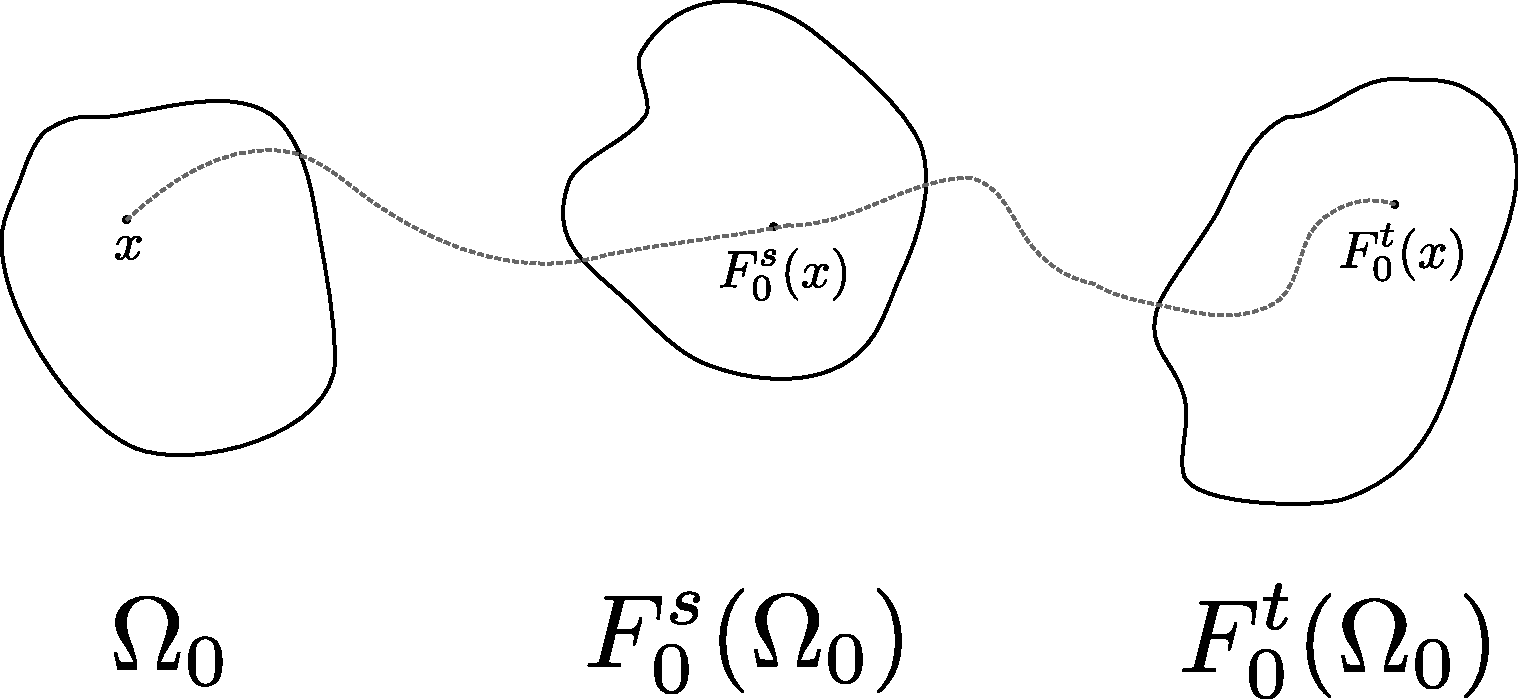
\includegraphics[width=\textwidth]{chp02_background/figures/flow_map.pdf}
		\caption{A pictorial representation of the flow map \(F\) corresponding to a continuous time dynamical system.}
		\label{fig:flow_map_diag}
	\end{center}
\end{figure}

The flow map satisfies the following properties, under ASSUMPTIONS?
For any \(r, s, t \in [0,T]\) and points \(x,w \in \R^n\),
\begin{enumerate}
	\item \(F_{s}^{t}\) is invertible with inverse
	      \[
		      \left[F_{s}^{t}\right]^{-1}\left(w\right) = F_{t}^{s}\left(w\right).
	      \]
	\item \(F_s^{t}\left(F_{r}^{s}(x)\right) = F_{r}^{t}\left(x\right)\)
\end{enumerate}
Moreover, the gradient of the flow map (with respect to the initial condition) provides insight into the local behaviour of the dynamical system \citep{Arnold_1973_OrdinaryDifferentialEquations,TruesdellNoll_2004_NonLinearFieldTheories}.
This gradient	satisfies a useful property; the equation of variations.
\begin{theorem}
	Let \(F_{t_1}^{t}\) be the flow map corresponding to \eqref{eqn:det_ode}.
	Then, the spatial gradient \(\nabla F_{t_0}^t(x)\) satisfies the equation of variations
	\begin{equation}
		\dpd{\nabla F_{t_1}^{t}(x)}{t} = \nabla u\left(F_{t_1}^{t}(x), t\right) \nabla F_{t_1}^{t}(x).
		\label{eqn:eqn_of_variations}
	\end{equation}
\end{theorem}
\begin{proof}
	Taking the gradient on both sides of \eqref{eqn:flow_map_ode} and using the chain rule gives
	\[
		\nabla\left(\dpd{F_{t_1}^{t_2}(x)}{t}\right) = \nabla u\left(F_{t_1}^{t}(x), t\right) \nabla F_{t_1}^{t}(x).
	\]
	Since the flow map is sufficiently smooth, we can interchange the derivatives on the right-hand side to arrive at
	\[
		\dpd{\nabla F_{t_1}^{t}(x)}{t} = \nabla u\left(F_{t_1}^{t}(x), t\right) \nabla F_{t_1}^{t}(x),
	\]
	as required.
\end{proof}



An important inequality for establishing bounds

\begin{theorem}[Gr\"onwall's inequality]\label{thm:gronwall}
	Let \(\alpha, \beta, u: [a,b] \to \R\) be functions such that \(\beta\) and \(u\) are continuous and that the negative part of \(\alpha\) is integrable on every closed and bounded subset of \([a,b]\).
	Then, if \(\beta\) is non-negative and for all \(t \in [a,b]\),
	\[
		u(t) \leq \alpha(t) + \int_a^t{\beta(\tau)u(\tau)\dif\tau}
	\]
	then
	\[
		u(t) \leq \alpha(t) + \int_a^t{\alpha(\tau)\beta(\tau)\exp\left(\int_\tau^{t}{\beta(s)\dif s}\right)\dif\tau}.
	\]
	Additionally, if \(\alpha\) is non-decreasing, then
	\[
		u(t) \leq \alpha(t) \exp\left(\int_a^t{\beta(\tau)\dif\tau}\right)
	\]
\end{theorem}
\begin{proof}

\end{proof}


\section{Notions of probabilistic convergence}
There are several different notions of convergence for a sequence of random variables, which we briefly recall here.
Consider a sequence of \(m\)-dimensional random vectors \(X_1, X_2,\dotsc\) and an \(m\)-dimensional random vector \(X\).
We say that:
\begin{itemize}
	\item The sequence \(X_1, X_2, \dotsc\) converges \emph{in distribution} to \(X\) if
	      \[
		      \lim_{n\to\infty}F_n\left(x\right) = F(x),
	      \]
	      where \(F_n\) is the cumulative distribution function for \(X_n\) and \(F\) is the cumulative distribution function for \(X\), for every point \(x \in \R^m\) where \(F\) is continuous.
	      If this is the case, we write
	      \[
		      X_n \xlongrightarrow[\text{distribution}]{} X, \quad \text{as } n \to \infty.
	      \]
	      Note that the limiting random vector \(X\) need not be defined on the same probability space as the terms in the sequence \(X_1, X_2, \dotsc\); convergence in distribution is the only notion of convergence for which this is the case.


	\item The sequence \(X_1, X_2, \dotsc\) converges \emph{in probability} to \(X\) if for every \(\delta > 0\)
	      \[
		      \lim_{n\to\infty}P\left(\norm{X_n - X} < \delta\right) = 0,
	      \]
	      in which case we write
	      \[
		      X_n \xlongrightarrow[\text{probability}]{} X, \quad \text{as } n \to \infty.
	      \]

	\item The sequence \(X_1, X_2, \dotsc\) converges \emph{almost surely} to \(X\) if
	      \[
		      P\left(\lim_{n \to \infty}X_n = X\right) = 1,
	      \]
	      in which case we write
	      \[
		      X_n \xlongrightarrow[\text{almost surely}]{} X, \quad \text{as } n \to \infty.
	      \]

	\item For \(r > 0\), the sequence \(X_1, X_2, \dotsc\) converges \emph{in \(r\)th mean} to \(X\) if
	      \[
		      \lim_{n\to\infty}{\avg{\norm{X_n - X}^r}} = 0,
	      \]
	      in which case we write
	      \[
		      X_n \xlongrightarrow[r\text{th mean}]{} X, \quad \text{as } n \to \infty.
	      \]
	      This type of convergence is also known as \emph{\(L_r\)-convergence}, as it corresponds to convergence in the \(L_r\) norm on the probability space on which \(X_1,\dotsc, X_n\) and \(X\) are defined.

\end{itemize}
There are implications between each notion of convergence, with convergence almost surely being the strongest and convergence in distribution the weakest.
These implications are summarised in \Cref{fig:rv_conv_impl}.

\usetikzlibrary{positioning}
\begin{figure}
	\begin{center}
		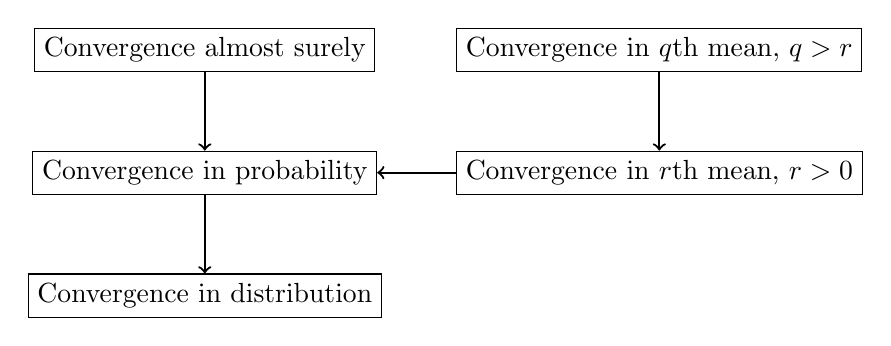
\begin{tikzpicture}
			\node (as) [draw] {Convergence almost surely};
			\node (p) [draw, below=of as] {Convergence in probability};
			\node (rm) [draw, right=of p] {Convergence in \(r\)th mean, \(r > 0\)};
			\node (qm) [draw, above=of rm] {Convergence in \(q\)th mean, \(q > r\)};
			% \node (rmom) [draw, below=of rm] {Convergence of \(r\)th moment};
			\node (d) [draw, below=of p] {Convergence in distribution};
			\path[->,thick] (as) edge  (p)
			(p) edge  (d)
			(qm) edge (rm)
			(rm) edge (p);
			% (rm) edge (rmom);
		\end{tikzpicture}
		\caption{The strength of each notion of convergence in probability, where each directed arrow corresponds to an implication.
			These results are stated and proven in \citet{Bremaud_2020_ProbabilityTheoryStochastic}, for instance.}
		\label{fig:rv_conv_impl}
	\end{center}
\end{figure}



\section{Stochastic differential equations}
In practice, there is uncertainty associated with a differential equation, which may arise from a variety of sources including observational error, parameter uncertainty, interpolation error and due to unresolved effects in the model.
Stochastic differential equations are an extension of ordinary differential equations that include stochastic terms, which can account for this uncertainty.
For a formal introduction to stochastic differential equations, see \citet{Oksendal_2003_StochasticDifferentialEquations} or \citet{KallianpurSundar_2014_StochasticAnalysisDiffusion}, for instance.
Here, we aim to only provide a brief overview and state theoretical results that prove relevant and useful in this thesis.
The following motivation of stochastic differential equations follows a similar one available in \citet{Oksendal_2003_StochasticDifferentialEquations}.

Suppose we have a deterministic dynamical system
\[
	\dod{x_t}{t} = u\left(x_t, t\right)
\]
where there is some uncertainty associated with the vector field \(u\).
In lieu of any additional understanding of this uncertainty, we model it as a stochastic noise.
Ideally, we would parameterise the uncertainty with some continuous-time stochastic process \(\xi_t\!\left(x_t\right)\), and write
\[
	\dod{y_t}{t} = u\left(x_t, t\right) + \xi_t\!\left(x_t\right).
\]
The noise process \(\xi_t\) can depend on the state, since we may expect that the magnitude and structure of the uncertainty varies with both the state and time.


Additionally, since we are modelling with a continuum, the noise process \(\xi_t\) should be (with probability \(1\)) continuous in time.
However, such a noise process \(\xi_t\) does not exist \citehere, in that there is no continuous process with properties 1 to 4, so we need an alternative formulation of the integral.
This leads to the It\^o integral, and It\^o stochastic differential equations.



\subsection{The Wiener process}
Before we define the It\^o integral, we must first establish what our driving noise process looks like.
The Wiener process, or Brownian motion, is an example of a continuous-time stochastic process that is often used to model \td{something}
Defined formally, the (one-dimensional) \emph{Wiener process} is a stochastic process \(B_t\) taking values in \(\R\) and satisfying the following properties:
\begin{romanate}
	\item \(B_0 = 0\),
	\item for every \(s > 0\), the increments \(B_{s + t} - B_{s}\) for \(t \geq 0\) are independent of \(B_r\) for all \(r < s\),
	\item \(B_{s + t} - B_t \isGauss{0, s}\) for all \(s,t > 0\), and
	\item \(B_t\) is continuous in \(t\) almost surely.
\end{romanate}
Remarkably, these properties \emph{uniquely} define the Wiener process, with the additional result that for any \(t > 0\), \(B_t \sim \mathcal{N}\left(0, t\right)\), a Gaussian distribution with mean zero and variance \(t\).
The \emph{\(n\)-dimensional Wiener process} is a stochastic process \(W_t\) taking values in \(R^n\) such that each component of \(W_t\) is a one-dimensional Wiener process and the components of \(W_t\) are mutually independent.
It follows that for the \(n\)-dimensional Wiener process \(W_t\), at any time \(t > 0\), \(W_t \sim \mathcal{N}\left(0, tI\right)\), an \(n\)-dimensional Gaussian distribution with mean zero and covariance matrix \(tI\).

A Wiener process is a type of L\'evy process, which is a more general class of stochastic process satisfying only conditions (i), (ii), and (iii) above \citep{Applebaum_2004_LevyProcessesStochastic}.



\subsection{The It\^o integral}
\td{Some sort of motivation or introduction}
For our purposes, we can think of an It\^o integral as being defined as the limit in probability of a sequence of sums, i.e. for a scalar but possibly random-valued function \(f\colon [a,b] \to \R\),
\begin{equation}\label{eqn:ito_int_limit_defn}
	\sum_{\left[t_i, t_{i+1}\right] \in \mathcal{P}_N}{f\left(t_{i}\right)\left(W_{t_{i+1}} - W_{t_i}\right)} \xlongrightarrow[\text{probability}]{} \int_a^b{f(t)\dif W_t}, \quad \text{as } N \to \infty
\end{equation}
where \(\mathcal{P}_N\) is a partition of \(\left[a,b\right]\) with \(\lim_{N \to \infty}\mathcal{P}_N = [a,b]\), \emph{\`a la} the definition of the Riemann integral.
It can be shown that this limit exists for a large class of both deterministic- and random-valued functions, by constructing appropriate approximations of the function \(f\).
This construction of the It\^o integral is available in many textbooks on stochastic processes, such as \citet{KallianpurSundar_2014_StochasticAnalysisDiffusion} and \citet{Oksendal_2003_StochasticDifferentialEquations}, so it will not be repeated here.

The extension of the It\^o integral to vector- and matrix-valued functions is straightforward.
Let \(g \colon [a,b] \to \R^{n \times m}\) be a function giving possibly random \(n \times m\) matrices (take \(m = 1\) to describe a vector-valued function).
\begin{subequations}\label{eqn:mv_ito_defn}
	Then, we define the It\^o integral of \(g\) with respect to the \(m\)-dimensional Wiener process \(W_t\) over the time interval \([a,b]\) as
	\begin{equation}\label{eqn:mv_ito_defn_1}
		\int_a^b{g(t)\dif W_t} \coloneqq \left(\mathcal{I}_1, \dotsc, \mathcal{I}_n\right)^{\T},
	\end{equation}
	where
	\begin{equation}\label{eqn:mv_ito_defn_2}
		\mathcal{I}_{i} = \sum_{j=1}^m{\int_a^b{g_{ij}\left(t\right) \dif W_t^{(j)}}},
	\end{equation}
	for \(i = 1,\dotsc, n\) and where \(g_{ij}\) denotes the \((i,j)\)th element of \(g\).
\end{subequations}

\subsection{It\^o stochastic differential equations}
The differential form of an \(n\)-dimensional It\^o stochastic differential equation is
\begin{equation}
	\dif y_t = u\left(y_t, t\right)\dif t + \sigma\left(y_t, t\right)\dif W_t,
	\label{eqn:gen_sde}
\end{equation}
where the solution \(y_t\) is a stochastic process taking values in \(\R^n\), \(u\colon \R^n \times \R \to \R^n\) is the drift and \(\sigma\colon \R^n \times \R \to \R^{n\times m}\) is the diffusivity.
The driving process \(W_t\) is the \(m\)-dimensional Wiener process.
For a (possibly random) initial condition \(y_0\), the solution \(y_t\) to \eqref{eqn:gen_sde} satisfies
\begin{equation}
	y_t = y_0 + \int_0^t{u\left(y_\tau, \tau\right)\dif\tau} + \int_0^t{\sigma\left(y_\tau, \tau\right)\dif W_\tau}.
	\label{eqn:gen_sde_int}
\end{equation}
The terms of the differential form \eqref{eqn:gen_sde} are not all rigorously defined, and so the differential form is rather notation that is equivalent to \eqref{eqn:gen_sde_int}.
In the most general case, the drift \(u\) and diffusivity \(\sigma\) are permitted to themselves be random functions\footnote{For more information, see for instance \citet{KallianpurSundar_2014_StochasticAnalysisDiffusion}.
	The formal treatment of such stochastic differential equations remains an area of open research, such as establishing the conditions for existence and uniqueness of solutions \citehere, and EXAMPLE.}, but in this thesis we assume that both are deterministic.


As with ordinary differential equations, we are interested in knowing when a given stochastic differential equation has solutions, and when those solutions are unique.
Since we are now dealing with random processes,

The main distinction are that strong solutions are defined on the \emph{same} probability space as the given driving Wiener process, whereas weak solutions are defined on \emph{any} probability space with a possibly different Wiener process.
This leads to two different notion of uniqueness; a strong solution \(y_t\) is strongly (or pathwise) unique if for any other strong solution \(x_t\),
\[
	P\left(y_t = x_t \, \forall t \in [0,T]\right) = 1.
\]
If \(x_t\) was not defined on the same probability space as \(y_t\), then the probability of equality would not make sense.

For our purposes, the distinction between strong and weak solutions

We can now state the requirements for the existence of unique strong solutions to \eqref{eqn:gen_sde}, in the following theorem.

\begin{theorem}[Existence and Uniqueness of SDE Solutions]

\end{theorem}



\subsection{Additive versus multiplicative noise}
In a stochastic differential equation of the form \eqref{eqn:gen_sde}, the diffusion matrix \(\sigma\) dictates the form of the noise in the system, and how easily (if at all) an analytical solution can be found.

When \(\sigma\) only has time-dependence, and no dependence on the state, the noise is \emph{additive}.

When there is state-dependence in \(\sigma\), the noise is termed \emph{multiplicative}.


\subsection{Analytical tools for It\^o calculus}
There are several tools available for the analytic treatment of It\^o integrals and solutions to stochastic differential equations, which we make use of throughout.
The first is It\^o's isometry, which relates the expectation of an It\^o integral to that of a deterministic one and is useful for computing moments.
\begin{theorem}[It\^o's Isometry]\label{thm:ito_isom}
	Let \(f: \Omega \times [0,T] \to \R\) be an It\^o integrable stochastic process.
	Then, for any \(t \in [0,T]\)
	\[
		\avg{\left(\int_0^t{f\left(\omega, \tau\right)\dif W_\tau}\right)^2} = \avg{\int_0^t{f\left(\omega, \tau\right)^2\dif\tau}}
	\]
\end{theorem}
\begin{proof}
	It\^o's isometry typically arises in the formal construction of the It\^o integral.
	For example, see Section 5.1 of \citet{KallianpurSundar_2014_StochasticAnalysisDiffusion}.
\end{proof}

Next, we have It\^o's Lemma (or the It\^o Formula), which is a change-of-variables formula in stochastic calculus and can be thought of as a generalisation of the chain rule from deterministic calculus.
We state and use the multidimensional form of the Lemma for solutions to It\^o stochastic differential equations, although more general forms exist (e.g. see Theorem 5.4.1 of \citet{KallianpurSundar_2014_StochasticAnalysisDiffusion}).
\begin{theorem}[It\^o's Lemma]
	Let \(X_t\) be the strong solution to the stochastic differential equation
	\[
		\dif X_t = a\left(X_t, t\right)\dif t + b\left(X_t, t\right)\dif W_t,
	\]
	where \(a: \R^n \times [0,\infty) \to \R^n\), \(b: \R^n \times [0,\infty) \to \R^{n\times p}\) and \(W_t\) is the canonical \(p\)-dimensional Wiener process.
	If \(f: \R^n \times [0, \infty) \to \R^m\) is twice continuously-differentiable, then the stochastic process \(Y_t \coloneqq f\left(X_t, t\right)\) is a strong solution to the stochastic differential equation
	\begin{align*}
		\dif Y_t & = \left(\dpd{f}{t}\left(X_t, t\right) + \nabla f\left(X_t, t\right) a\left(X_t, t\right) + \frac12\mathrm{tr}\left[b\left(X_t, t\right)^{\T} \nabla\nabla f\left(X_t, t\right) b\left(X_t, t\right)\right] \right)\dif t \\
		         & \qquad\qquad\qquad\qquad + \nabla f\left(X_t, t\right)b\left(X_t, t\right) \dif W_t.
	\end{align*}
\end{theorem}
\begin{proof}

\end{proof}

Our third and final result is the Burkholder-Davis-Gundy inequality, which when applied to stochastic integrals provides bounds on the expected norm.
\begin{theorem}[Burkholder-Davis-Gundy Inequality]
	Let \(M_t\) be an It\^o-integrable stochastic process taking values in \(\R^n\).
	Then, for any \(p > 0\) there exists constants \(c_p, C_p > 0\) independent of the stochastic process \(M_t\) such that
	\[
		c_p\avg{\left(\int_0^t{\norm{M_\tau}^2\dif \tau}\right)^p} \leq \avg{\sup_{\tau \in \left[0, t\right]}\norm{\int_0^\tau{M_s\dif W_s}}^{2p}} \leq C_p\avg{\left(\int_0^t{\norm{M_\tau}^2\dif \tau}\right)^p}.
	\]
\end{theorem}
\begin{proof}
	This result is stated and proven as Theorem 5.6.3 of \citet{KallianpurSundar_2014_StochasticAnalysisDiffusion}.
\end{proof}



\subsection{The Stratonovich integral and Stratonovich SDEs}
The Stratonovich integral is an alternative definition of a stochastic integral \citehere, which is arises naturally from physically considerations \citep{}.
The Stratonovich integral can be written as the limit in \(2\)nd mean
\[
	\sum_{t_i, t_{i+1} \in \mathcal{P}_N}{\frac{f\left(t_{i+1}\right) - f\left(t_i\right)}{2}\left(W_{t_{i+1}} - W_{t_i}\right)} \xlongrightarrow[2\text{nd mean}]{} \int_a^{b}{f(t)\circ\dif W_t}, \quad \text{as } N \to \infty
\]
where \(\mathcal{P}_N\) is again a partition of \([a,b]\) and the \(\circ \dif W_t\) notation is used to distinguish the Stratonovich intepretation of the integral.
The Stratonovich integral is extended to vector-valued functions and a multivariable Wiener process in the same fashion as \eqref{eqn:mv_ito_defn}.
We can then write a Stratonovich stochastic differential equation
\begin{equation}
	\dif x_t = u\left(x_t, t\right)\dif t + \sigma\left(x_t, t\right)\circ \dif W_t
	\label{eqn:strat_sde}
\end{equation}
in completely the same way as an It\^o SDE.
In this thesis, we only consider It\^o stochastic differential equations in our theoretical developments, but there is a conversion between the two interpretations that requires modifying the drift term \(u\) of the SDE.
The Stratonovich SDE \eqref{eqn:strat_sde} is equivalent to the It\^o SDE \citehere
\begin{equation}
	\dif x_t = \left[u\left(x_t, t\right) + c\left(x_t, t\right)\right]\dif t + \sigma\left(x_t, t\right)\dif W_t,
	\label{eqn:strat_ito_conv}
\end{equation}
where \(c\left(x_t, t\right) = \left(c_1\left(x_t, t\right), \dotsc, c_n\left(x_t, t\right)\right)^T\) with
\[
	c_i\left(x_t, t\right) \coloneqq \mathrm{tr}\left(\left[\nabla\sigma_{i\cdot}\left(x_t, t\right)\right]^{\T}\sigma\left(x_t, t\right)\right),
\]
where \(\nabla \sigma_{i\cdot}\) denotes the Jacobian derivative of the \(i\)th row of \(\sigma\).


\subsection{The Fokker-Planck equation}


The probability density function \(\rho: \R^n \times [0,T] \to [0,\infty)\) for the solution to \eqref{eqn:gen_sde} at time \(t \in [0,T]\) is the solution to the corresponding Fokker-Planck equation \citep{Risken_2012_FokkerPlanckEquationMethods}
\begin{equation}
	\dpd{\rho}{t} = \frac12\nabla\cdot\nabla\cdot\left(\rho\sigma\sigma^{\T}\right) - \nabla\cdot\left(\rho u\right)
	\label{eqn:fp_eqn}
\end{equation}
subject to some initial density \(\rho\left(x,0\right)\) given by the initial condition to \eqref{eqn:gen_sde}.
To ensure that the solution is a valid probability density function on \(\R^n\), for any \(t \in [0,T]\), \(\rho\) must satisfy
\begin{subequations}\label{eqn:fp_valid_pdf}
	\begin{align}
		\int_{\R^n}{\rho\left(x, t\right)\dif x} = 1, \label{eqn:fp_valid_pdf_norm} \\
		\lim_{x \to \infty}\rho\left(x,t\right) = 0. \label{eqn:fp_valid_pdf_limit}
	\end{align}
\end{subequations}
For a fixed and deterministic initial condition \(y_0 = x\), the corresponding initial condition to \eqref{eqn:fp_eqn} is the Dirac-delta distribution centred at \(x\).

For certain choices of the drift \(u\) and diffusivity \(\sigma\), \eqref{eqn:fp_eqn} reduces to several other well-known partial differential equations, including:
\begin{itemize}
	\item When \(\sigma \equiv D\), a scalar constant, then \eqref{eqn:fp_eqn} is the convection-diffusion equation with velocity field \(u\) and diffusivity \(D\).

	\item When \(\sigma \equiv 0\), i.e. there is no diffusion, then \eqref{eqn:fp_eqn} is the continuity equation with velocity field \(u\).

\end{itemize}
The connection between the Fokker-Planck equation and the SDE \eqref{eqn:gen_sde} means that the solutions to each of these PDEs can be equivalently thought of as the time-evolution of the probability density of an SDE.


The Fokker-Planck equation is linear, so we can apply a technique known as Green's function method (for an example of this approach on a linear SDE, see Section 3.2 of \citet{Risken_2012_FokkerPlanckEquationMethods}) in order to understand the behaviour of solutions with non-fixed initial conditions.
Let \(\mathcal{P}_t\set{\rho_0}\) denote the solution operator of \eqref{eqn:fp_eqn} with initial density \(\rho_0\colon \R^n \to \R^n\).
Then, since \eqref{eqn:fp_eqn} is a linear equation, \(\mathcal{P}_t\) is a linear operator.
Now, let \(x_0 \in \R^n\) be an arbitrary fixed point, and consider the fundamental solution, or Green's function,
\[
	G_t\left(x; x_0\right) \coloneqq \mathcal{P}_t\set{\delta_{x_0}}\!\left(x\right).
\]
That is, \(G_t\left(x; x_0\right)\) is the solution to the Fokker-Planck equation with the Dirac-delta initial condition \(\delta_{x_0}(x) = \delta\left(x - x_0\right)\), which is equivalent to the SDE \eqref{eqn:gen_sde} with the deterministic and fixed initial condition \(y_0 = x_0\).
The Green's function \(G_t\) is equivalently the transition probability function of the SDE solution \(x_t\) as a stochastic process.
Now, using the sampling property of the Dirac-delta function, for a general initial density \(\rho_0\colon \R^n \to \R^n\),
\[
	\rho_0(x_0) = \int_{\R^n}{\rho_0\left(x\right)\delta_{x_0}\left(x\right)\dif x}.
\]
Since \(\mathcal{P}_t\) is linear,
\begin{equation}
	\mathcal{P}_t\set{\rho_0}\!\left(x_0\right) = \int_{\R^n}{\rho_0\left(x\right)\mathcal{P}_t\set{\delta_{x_0}}\!\left(x\right)\dif x} = \int_{\R^n}{\rho_0\left(x\right) G_t\left(x; x_0\right)\dif x}.
	\label{eqn:fp_greens_trick}
\end{equation}




% \section{Aspects of stochastic parameterisation}
% When using deterministic systems to model real-world phenomena, there are many ways in which uncertainty can arise.
% For instance,

% Stochastic parameterisation is a
% These unresolved subgrid effects are accounted for by introducing stochastic noise into the otherwise deterministic model.

% \citet{BernerEtAl_2017_StochasticParameterizationNew}

% \citet{LeutbecherEtAl_2017_StochasticRepresentationsModel}

% \subsection{Additive versus multiplicative noise}

% When \(\sigma = \sigma(t)\) depends only on \(t\), then noise is considered \emph{additive}.
% If there is spatial dependence in \(\sigma\), i.e. \(\sigma = \sigma(x,t)\), then the noise considered \emph{multiplicative}.



% For instance, \citet{SuraEtAl_2005_MultiplicativeNoiseNonGaussianity} shows that the non-Gaussian statistics observed in atmospheric regimes can arise from linear models with multiplicative noise.



\subsection{Some explicitly solvable SDEs}\label{sec:back_sde_solutions}
In general, the solution to a stochastic differential equation cannot be expressed analytically, either as an explicit expression involving the Wiener process \(W_t\) or as a probability measure or density function.
At best, most solutions can be written in terms of an It\^o integral which can otherwise not be simplified.
However, there are several simple examples for which a solution can be written, and even time-marginal probability density functions can be derived.
Here, we list several examples which are used to validate theory and test algorithms throughout this thesis.

\begin{example}[Homogenous and linear SDE]
	Consider an \(n\)-dimensional stochastic differential equation
	\begin{equation}
		\sde{x_t}{A(t)x_t}{B(t)},
		\label{eqn:linear_sde}
	\end{equation}
	where \(A\colon [0,T] \to \R^{n\times n}\) is an matrix-valued function where each element is differentiable, and \(B\colon [0,T] \to \R^{n\times m}\) is a matrix-valued function, and \(W_t\) is an \(m\)-dimensional Wiener process.
	The weak solution to \eqref{eqn:linear_sde} is a Gaussian process, given at time \(t\) by
	\[
		x_t \isGauss{\Phi(t) x_0, \, \Phi\left(t\right)\left[\int_0^t{\Phi\left(\tau\right)^{-1}B\left(t\right)B\left(t\right)^{\T}\left(\Phi\left(\tau\right)^{-1}\right)^{\T}}\right]\Phi(t)^{\T}},
	\]
	where \(\Phi\) is the fundamental matrix solution to the corresponding homogeneous equation
	\[
		\dod{\Phi(t)}{t} = A(t)\Phi(t).
	\]
	The details of this result are provided in \Cref{app:linear_sde_sols}.
	When the coefficients \(A\) and \(B\) are constant functions, then the solution to \eqref{eqn:linear_sde} is also known as an Ornstein-Uhlenbeck process.

\end{example}

\begin{example}[Ben\^e's SDE]\label{ex:bene_sde}
	The \(1\)-dimensional stochastic differential equation
	\begin{equation}
		\sde{x_t}{\tanh\left(x_t\right)}{},
		\label{eqn:bene_sde}
	\end{equation}
	is known as \emph{Ben\^e's stochastic differential equation} \citep{SarkkaSolin_2019_AppliedStochasticDifferential}.
	The probability density function of a weak solution of \eqref{eqn:bene_sde} can be derived using an appropriate change of measure with Girsanov's theorem.
	A proof of this, and the derivation of a weak solution to \eqref{eqn:bene_sde} are provided in Section 7.3 of \citet{SarkkaSolin_2019_AppliedStochasticDifferential}.
	The probability density function \(p: \R \times \left(0,\infty\right) \to \left[0,\infty\right)\) for the solution \(x_t\) at time \(t > 0\) is given by
	\begin{equation}\label{eqn:bene_sde_pdf}
		p(x,t) = \frac{1}{\sqrt{2\pi t}}\frac{\cosh\left(x\right)}{\cosh\left(x_0\right)}\exp\left[-\frac{t}{2} - \frac{1}{2t}\left(x - x_0\right)^2\right],
	\end{equation}
	where \(x_0 \in \R\) is a fixed initial condition.
	For fixed \(t\), the probability density function can be expressed as the mixture of two Gaussian densities with variance \(t\) and respective means \(x_0 + t\) and \(x_0 - t\), i.e.
	\[
		p(x,t) = \frac{1}{2\cosh\left(x_0\right)}\left[\exp\left(x_0\right)\mathcal{N}\!\left(x; x_0 + t, t\right) + \exp\left(-x_0\right)\mathcal{N}\!\left(x; x_0 - t, t\right)\right],
	\]
	with details provided in \Cref{app:bene_calculations}.
	This probability density function is plotted, for the initial condition \(x_0 = 1/2\) and various times, in \Cref{fig:bene_pdf}.
	The resulting density is not symmetric and bimodal, with the two modes moving apart in the positive and negative \(x\)-directions respectively as \(t\) increases.
	% This expression allows easy calculation of the mean and expectation of \(x_t\), as
	% \[
	% 	\avg{x_t} = \frac{x_0\cosh\left(x_0\right) + t\sinh\left(x_0\right)}{\cosh\left(x_0\right)},
	% \]
	% and
	% \[
	% 	\var{x_t} =
	% \]
\end{example}


\newcommand{\plotbenepdf}[2]{
	\begin{tikzpicture}\begin{axis}[
				ymin=0.0,
				xmin=-10.0,
				xmax=10.0,
				axis lines=center,
				axis on top=true,
				domain=-10:10,
				ylabel=$p$,
				xlabel=$x$,
				ytick=\empty,
				yticklabels={},
			]
			\addplot [mark=none,draw=black,thick,samples=500] {cosh(\x)*exp(-#2/2-1/(2 * #2)*(\x-#1)^2)/((2 * pi * #2)^(1/2) * cosh(#1))};
		\end{axis}
	\end{tikzpicture}
}

\begin{figure}
	\begin{center}
		\begin{subfigure}{0.49\textwidth}
			\plotbenepdf{1/2}{1}
			\caption{\(t = 1\)}
			\label{fig:bene_1}
		\end{subfigure}
		\begin{subfigure}{0.49\textwidth}
			\plotbenepdf{1/2}{2.5}
			\caption{\(t = 2.5\)}
			\label{fig:bene_2.5}
		\end{subfigure}
		\begin{subfigure}{0.49\textwidth}
			\plotbenepdf{1/2}{5}
			\caption{\(t = 5\)}
			\label{fig:bene_5}
		\end{subfigure}
		\begin{subfigure}{0.49\textwidth}
			\plotbenepdf{1/2}{7.5}
			\caption{\(t = 7.5\)}
			\label{fig:bene_7.5}
		\end{subfigure}
	\end{center}
	\caption{The probability density function \eqref{eqn:bene_sde_pdf} for the time-marginal solution of Ben\^e's SDE \eqref{eqn:bene_sde}, for the initial condition \(x_0 = 1/2\) at various times.
		The density function consists of two distinct modes that move further apart as \(t\) increases.}
	\label{fig:bene_pdf}
\end{figure}




\subsection{Numerical schemes for approximating SDEs}
In general, solving a stochastic differential equation analytically is not possible, and so as with ordinary differential equations we instead look to use numerical schemes to approximate solutions.
However, the solution to a stochastic differential equation is itself a random variable, so a single sample path is not sufficient.
Instead, a numerical SDE scheme produces approximate \emph{realisations} of the solution.
The Euler-Maruyama (EM) method is analogous to the Euler method for ODEs, and considered by many to be the simplest method for numerically solving SDEs \citep{KloedenPlaten_1992_NumericalSolutionStochastic}.
The update step of the EM scheme, with step size \(\Delta t\), is
\begin{equation}
	\hat{x}_{t + \Delta t} = \hat{x}_{t} + \Delta t u\left(\hat{x}_t, t\right) + \Delta t \sigma\left(\hat{x}_t, t\right) Z_t,
	\label{eqn:em_step}
\end{equation}
where \(Z_t\) is sampled from the standard Gaussian \(\Gauss{0,I}\), and the scheme is initialised as \(\hat{x}_0 = x_0\).
The Euler-Maruyama scheme has strong order 0.5, meaning that
\[
	\avg{\norm{x_t - \hat{x}_{t}\left(\Delta t\right)}} = \mathcal{O}\left(\Delta t^{0.5}\right),
\]
where \(\hat{x}_t\left(\Delta t\right)\) is the Euler-Maruyama estimate at time \(t\) using step size \(\Delta t\).


There are many other schemes for generating approximate samples of a stochastic differential equation, of varying weak and strong orders.
For instance, extensions of Runge-Kutta-type schemes \citep{Roberts_2012_ModifyImprovedEuler,Rossler_2010_RungeKuttaMethodsStrong}.



\section{Stochastic sensitivity}
To address the need for computational tools that quantify uncertainty without,

This work directly addressed the emerging need to explicit quantify the impact of velocity uncertainty on Lagrangian trajectories \citep{Balasuriya_2020_StochasticApproachesLagrangian,BalasuriyaGottwald_2018_EstimatingStableUnstable,BranickiUda_2021_LagrangianUncertaintyQuantification,HallerEtAl_2018_MaterialBarriersDiffusive}.


Given possibly time-dependent velocity data \(u: \R^2 \times [0,T] \to \R^2\), \citet{Balasuriya_2020_StochasticSensitivityComputable} considers the evolution of solutions to the differential equation
\[
	\dod{x_t}{t} = u\left(x_t, t\right).
\]
Solutions can be summarised by the flow map \(F_{t_1}^{t_2}\), as in \Cref{def:flow_map}.
In most practical situations, the Eulerian velocity data driving ocean and atmospheric models relies upon measurements of estimates obtained on a low resolution spatial discretisation.
\citet{Balasuriya_2020_StochasticSensitivityComputable} introduces stochastic sensitivity as a new tool for directly quantifying the impact of Eulerian uncertainty on Lagrangian trajectories.
The evolution of Lagrangian trajectories is modelled as solution to a It\^o stochastic ordinary differential equation.

To directly account for these unresolved sources of uncertainty, the ``true'' Lagrangian trajectories evolve as solution to the stochastic differential equation
\begin{equation}
	\sde{y_t}{u\left(y_t, t\right)}{\epsilon\sigma\left(y_t, t\right)},
	\label{eqn:ss_sde},
\end{equation}
where \(0 < \epsilon \ll 1\) is a parameter quantifying the scale of the noise, \(\sigma:	\R^2\times[0,T] \to \R^{2\times 2}\) is the \(2\times 2\) diffusion matrix, and \(W_t\) is the canonical two-dimensional Wiener process.
In the original formulation \citep{Balasuriya_2020_StochasticSensitivityComputable}, \(\epsilon\) is a dimensionless parameter and \(\sigma\) is dimensional, but an alternative scaling technique relates \(\epsilon\) to spatial and velocity uncertainty scales in the data (see the follow-up work by \citet{BadzaEtAl_2023_HowSensitiveAre,Balasuriya_2020_UncertaintyFinitetimeLyapunov,FangEtAl_2020_DisentanglingResolutionPrecision})
Since \(\sigma\) can vary by both space and time, the noise is multiplicative.
The diffusion matrix \(\sigma\) is specified \emph{a priori}, based on any knowledge of how uncertainty varies with space and time, e.g. from experimental considerations, observation error estimates.
If no such prior information is known, then \(\sigma \equiv I\), the \(2 \times 2\) identity matrix is the default choice.

To quantify uncertainty in a way that is independent of the noise scale \(\epsilon\), \citet{Balasuriya_2020_StochasticSensitivityComputable} defined the random variable \(z_\epsilon\left(x,t\right)\) on \(\R^2 \times [0,T]\) as
\[
	z_\epsilon\left(x,t\right) \coloneqq \frac{y_t - F_0^t(x)}{\epsilon}.
\]
The main aim is to compute statistics of \(z_\epsilon\) at the final time \(T\), so that of \(z_\epsilon\left(x,T\right)\).
\citet{Balasuriya_2020_StochasticSensitivityComputable} then considers the signed projection of \(z_\epsilon\left(x,T\right)\) onto a ray emanating from the deterministic position \(F_0^T(x)\) in a given direction, defining
\[
	P_\epsilon\left(x,\theta\right) \coloneqq \hat{n}^{\T} z_\epsilon(x,T),
\]
where \(\theta \in \left[-\pi/2, \pi/2\right)\) and
\[
	\hat{n}(\theta) = \begin{bmatrix}
		\cos{\theta} \\
		\sin{\theta}
	\end{bmatrix}.
\]


The statistics of \(z_\epsilon\left(x,T\right)\) and \(P_\epsilon(x,\theta)\) are considered in the limit as \(\epsilon\downarrow 0\), which provides a characterisation of the uncertainty of the model \emph{independently} of the scale of the noise.
\citet{Balasuriya_2020_StochasticSensitivityComputable} provided computable expressions for the mean and variance of \(P_\epsilon\left(x,\theta\right)\) in this limit of small noise, which we summarise here.
For proofs of these results, see the appendices of \citet{Balasuriya_2020_StochasticSensitivityComputable}.

The first result established by \citet{Balasuriya_2020_StochasticSensitivityComputable} is that the expected location is deterministic, in the following sense.
\begin{theorem}[\citealt{Balasuriya_2020_StochasticSensitivityComputable}]
	For all \(x \in \R^2\),
	\[
		\lim_{\epsilon\downarrow 0}\avg{z_\epsilon(x,T)} = 0.
	\]
\end{theorem}

The variance of \(P_\epsilon\left(x,\theta\right)\) is used to assign a computable scalar measure of uncertainty to the trajectory.

\begin{definition}[\citealt{Balasuriya_2020_StochasticSensitivityComputable}]
	\begin{alpharate}
		\item The \textbf{anisotropic uncertainty} is a scalar field \(A: \R^2\times\left[-\pi/2, \pi/2\right) \to [0,\infty)\) defined by
		\[
			A(x,\theta) \coloneqq \sqrt{\lim_{\epsilon\downarrow 0}\var{P_\epsilon(x,\theta)}}.
		\]

		\item The \textbf{stochastic sensitivity} is a scalar field \(S: \R^2 \to [0,\infty)\) defined by
		\[
			S^2(x) \coloneqq \lim_{\epsilon\downarrow 0}\sup_{\theta}{\var{P_\epsilon(x,\theta)}}.
		\]
	\end{alpharate}
\end{definition}

By employing techniques from both deterministic and stochastic calculus (i.e. Gr\"onwall's inequality, the Burkholder-Davis-Gundy inequality, It\^o's Lemma), Balasuriya further established expressions for both the anisotropic uncertainty and the stochastic sensitivity that are computable given only the flow map and velocity data.

\begin{theorem}[\citealt{Balasuriya_2020_StochasticSensitivityComputable}]\label{thm:orig_s2_calculation}
	For \(x \in \R^2\), set \(w \coloneqq F_0^t(x)\).
	Then, for any \(\theta \in \left[-\pi/2, \pi/2\right)\),
	\[
		A(x,\theta) = \left(\int_0^T{\norm{\Lambda\left(x, t, T\right)J\hat{n}(\theta)}\dif t}\right)^{1/2},
	\]
	where
	\[
		\Lambda\left(x,t,T\right) \coloneqq e^{\int_t^T{\left[\nabla \cdot u\right]\left(F_0^\xi(x), \xi\right)\dif\xi}}\sigma\left(F_0^t(x), t\right)^{\T}J \nabla_w F_T^t\left(w\right),
	\]
	with the gradients \(\nabla_w\) of the flow map taken with respect to the mapped position \(w\), and
	\[
		J \coloneqq \begin{bmatrix}
			0 & -1 \\
			1 & 0
		\end{bmatrix}
	\]
	Additionally, stochastic sensitivity is computed as
	\[
		S^2(x) = P(x) + N(x),
	\]
	with
	\begin{align*}
		L(x) & \coloneqq \frac12\sum_{i=1}^2\int_0^T\left[\Lambda_{i2}\left(x,t, T\right)^2 - \Lambda_{i1}\left(x,t,T\right)^2\right]\dif t \\
		M(x) & \coloneqq \sum_{i=1}^2\int_0^T{\Lambda_{i1}\left(x,t,T\right)\Lambda_{i2}\left(x,t,T\right)\dif t}                           \\
		N(x) & \coloneqq \sqrt{L^2(x) + M^2(x)}                                                                                             \\
		P(x) & \coloneqq \abs{\frac12\sum_{i=1}^2\sum_{j=1}^2{\int_0^T{\Lambda_{ij}\left(x,t,T\right)^2\dif t}}},
	\end{align*}
	where \(\Lambda_{ij}\) is the \((i,j)\)-element of \(\Lambda\).
\end{theorem}




\begin{figure}
	\begin{center}
		\begin{subfigure}{0.8\textwidth}
			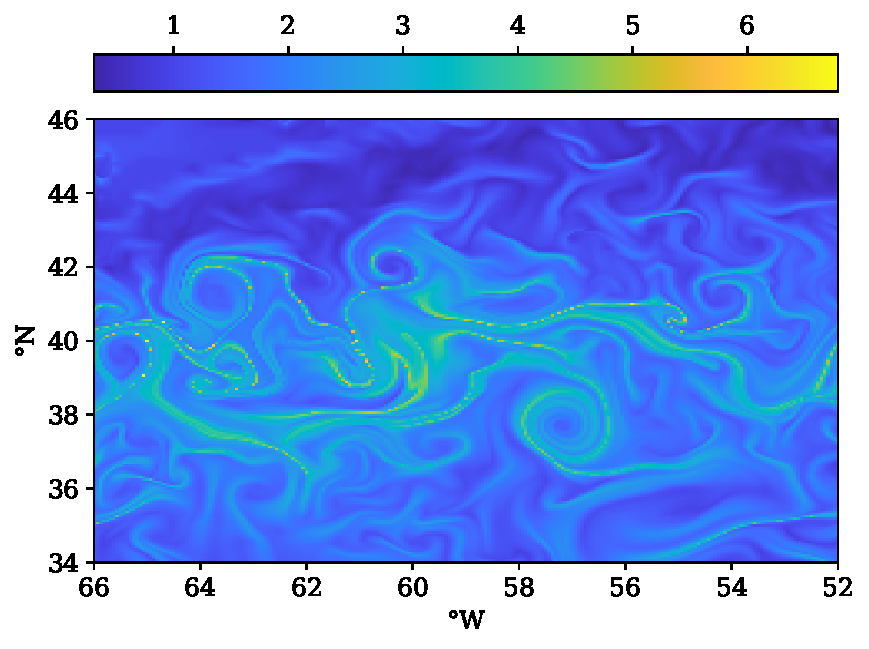
\includegraphics[width=\textwidth]{chp02_background/figures/res_scaled_stoch_sens_high_res.pdf}
			\caption{The resolution-scaled stochastic sensitivity field, plotted on a \(1/16\) degree resolution grid of initial conditions.}
			\label{fig:s2_na_ex_field}
		\end{subfigure}
		\begin{subfigure}{0.8\textwidth}
			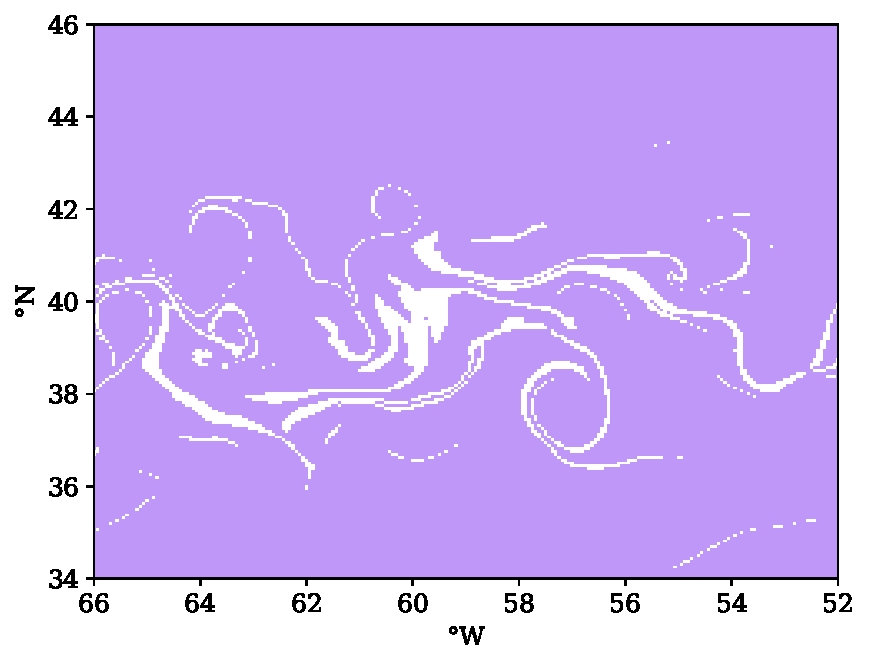
\includegraphics[width=\textwidth]{chp02_background/figures/robust_3.0_high_res.pdf}
			\caption{Robust sets (in purple) extracted from the stochastic sensitivity field in (a), using a lengthscale threshold of \(6\) degrees}
			\label{fig:s2_na_ex_sets}
		\end{subfigure}
		\caption{}
		\label{fig:fig:s2_na_ex}
	\end{center}
\end{figure}



Accordingly, \citet{Balasuriya_2020_StochasticSensitivityComputable} defines the \emph{resolution-scaled stochastic sensitivity} as
\begin{equation}
	S_r\left(x\right) \coloneqq \ln\left(\frac{\sqrt{S^2(x)}}{L_r}\right),
	\label{eqn:Sr_defn}
\end{equation}
where \(L_r\) is a specified spatial resolution lengthscale.
The \emph{noise-scaled stochastic sensitivity} is defined as
\begin{equation}
	S_n\left(x\right) \coloneqq \epsilon\sqrt{S^2(x)}.
	\label{eqn:Sn_defn}
\end{equation}

Stochastic sensitivity has also provided a novel approach to extracting Lagrangian coherent structures, which are regions of a fluid that remain ``coherent'' as the flow evolves over time \citep{BalasuriyaEtAl_2018_GeneralizedLagrangianCoherent,AllshousePeacock_2015_LagrangianBasedMethods,HadjighasemEtAl_2017_CriticalComparisonLagrangian}.

\Cref{fig:s2_na_ex_field} plots the resolution-scaled stochastic sensitivity field for a region of the North Atlantic ocean, including the Gulf Stream, as an illustrative example of how stochastic sensitivity is able to capture structures within a given flow.

% \begin{definition}[\citealt{Balasuriya_2020_StochasticSensitivityComputable}] \label{def:ss_res_scaled}
% 	Given a spatial resolution \(L_r\), the \emph{resolution-scaled stochastic sensitivity} is defined on \(\Omega\)
% 	\[
% 		S_r(x) \coloneqq \ln\left(\frac{\sqrt{S^2(x)}}{L_r}\right).
% 	\]
% \end{definition}
